\documentclass[a4paper,final]{article}
\usepackage{subfig}
\usepackage[dutch]{babel}
\usepackage{minutes}
\usepackage{graphicx}
\usepackage{float}

\title{Notulen 015 overleg team 33}
\author{Guus}
\minutesstyle{header=table, vote=list, contents=true, columns={1}}

\begin{document}
%\selectlanguage{dutch}

\begin{Minutes}{Overleg 014 team 33}
\participant{Face to face meeting Freek and Bernard}
\minutesdate{27 november 2014}
\location{Toernooiveld 200, Nijmegen (Mercator gebouw)}

\maketitle% This is where LaTeX makes the title

\topic{Introduction}

Bernard is promovendus op basis van derden geldstroom (Intel). Freek is
universitair docent. Als promovendus was NoC zijn onderwerp ( iets met
fabrics). Guus is OU student met een verleden in IT als programmeur,
functioneel en technisch ontwerper, informatie analist, en functioneel en
technisch beheer.

\paragraph{Rolverdeling} Zowel Bernard als Freek zijn actief bij het project
betrokken, maar conform onderlinge afspraak bemoeit Bernard zich naar ons toe
met de inhoud van het project en Freek met de begeleiding. 
Achter de schermen sluiten Freek en Bernard de inhoudelijke aspecten met elkaar kort.
De begeleiding is alleen zaak voor Freek.

Praktisch gezien is Freek meer gericht op de verificatie modules (bijvoorbeeld
deadlock detectie) terwijl Bernard gericht is op het hele project ten behoeve
van zijn promotie. 

\topic{Onderzoekscontext} Freek licht de doelen van het project toe. Enerzijds
zijn er onderzoekers aan de RU (Radboud Universiteit) die analyse en
verificatie tools maken en daar publicaties over doen.  Anderzijds willen de
onderzoekers hun publicaties aan de man brengen (``Valorisatie'') bij
onderzoekers bij andere universiteiten en bij bedrijven (zoals Intel). 

Voor onderzoekers maakt het ontwerp tool het mogelijk om de verificatie tools
(die in ontwikkeling zijn) snel te evalueren. Voor de buitenwereld
maakt het ontwerp tool de onderzoeken beter toegankelijk en 
maakt het onderzoek meer indruk in de wetenschappelijke wereld. 

\topic{Architectuur}

Het huidige tool heeft 2 fundamentele problemen. 

1. {\bf Het ontwerp tool is te ingewikkeld voor uitbreiding} en moeilijk voor
onderhoud. De interfaces en datastructuren lopen te ver uiteen met zelfs kleine
verschillen in semantiek. Er zijn te veel aparte oplossingen per onderzoeker.
Het huidige wicked xmas is te moeilijk onderhoudbaar.

2. {\bf Het ontwerp tool is te ingewikkeld om te installeren en gebruiken}. Dit
betekent dat het verspreiden en bekend maken van de verificatie tools veel
moeizamer verloopt.

Ons project moet aan beide problemen een einde maken.

\subtopic{Use cases}

\begin{itemize}

	\item Onderzoekers van de RU gebruiken het tool om hun verificatie tools te
		toetsen. Dat betekent dat de nieuwe tools gemakkelijk in het ontwerp
		tool in te passen moeten zijn. Dat betekent ook, dat het ontwerp tool
		niet weet hoe de verificatie tools werken.

		Opmerking van Bernard is om uitvoer van verificatie tools indien
		mogelijk via een stream te laten lopen, zodat het zowel op console als
		in een window kan verschijnen.

	\item Onderzoekers van andere universiteiten kunnen het tool voor
		ondersteuning van hun eigen onderzoek gebruiken. Ook hier weten we niet
		of zij de RU tools gebruiken of hun eigen tools ontwikkelen. Het maken
		en inpassen van een verificatie tool moet dus gemakkelijk zijn (user
		guide)

	\item Onderzoekers van externe bedrijven zoals Intel en ARM gebruiken het
		ontwerp tool voor het ontwerpen van NoC componenten. Een klein groepje
		Intel onderzoekers gebruikt het ook voor hun XMAS onderzoek. Daarnaast
		zijn deze onderzoekers ook geinteresseerd in de verificatie tools zelf.

	\item {\bf ter discussie} Onderzoekers kunnen hun werk willen delen met
		andere onderzoekers dan wel met studenten. Momenteel doet men dit door
		een bestand met het NoC ontwerp te repliceren via FTP of email. De
		vraag is of een C/S/ opzet hier hulp kan bieden. 

		Opmerking van Bernard is dat dit update C/S niet waarschijnlijk is.
		Read-only delen staat nog ter discussie.

	\item {\bf grotere netwerken} draaien vaker offline in batch mode. Hierbij
		komt alle uitvoer in bestanden terecht. Deze uitvoering van een run
		omvat dan alle verificatie tools.

	\item {\bf online} werken de onderzoekers waarbij zij selectief verificatie
		tools gebruiken en online eventuele parameters invoeren die voor de
		verificatie run nodig zijn.

	\item {\bf Toevoegen nieuwe tools}. De onderzoekers creeren nieuwe tools
		die zij toe voegen aan het bestaande arsenaal aan verificatie tools. De
		bedoeling is dat zij zich op de materie van hun tool kunnen
		concentreren zonder afleiding te vinden in de ``boilerplate'' code die
		voor integratie in het ontwerp nodig is. 

\end{itemize}		

\subtopic{Huidige en gewenste architectuur}

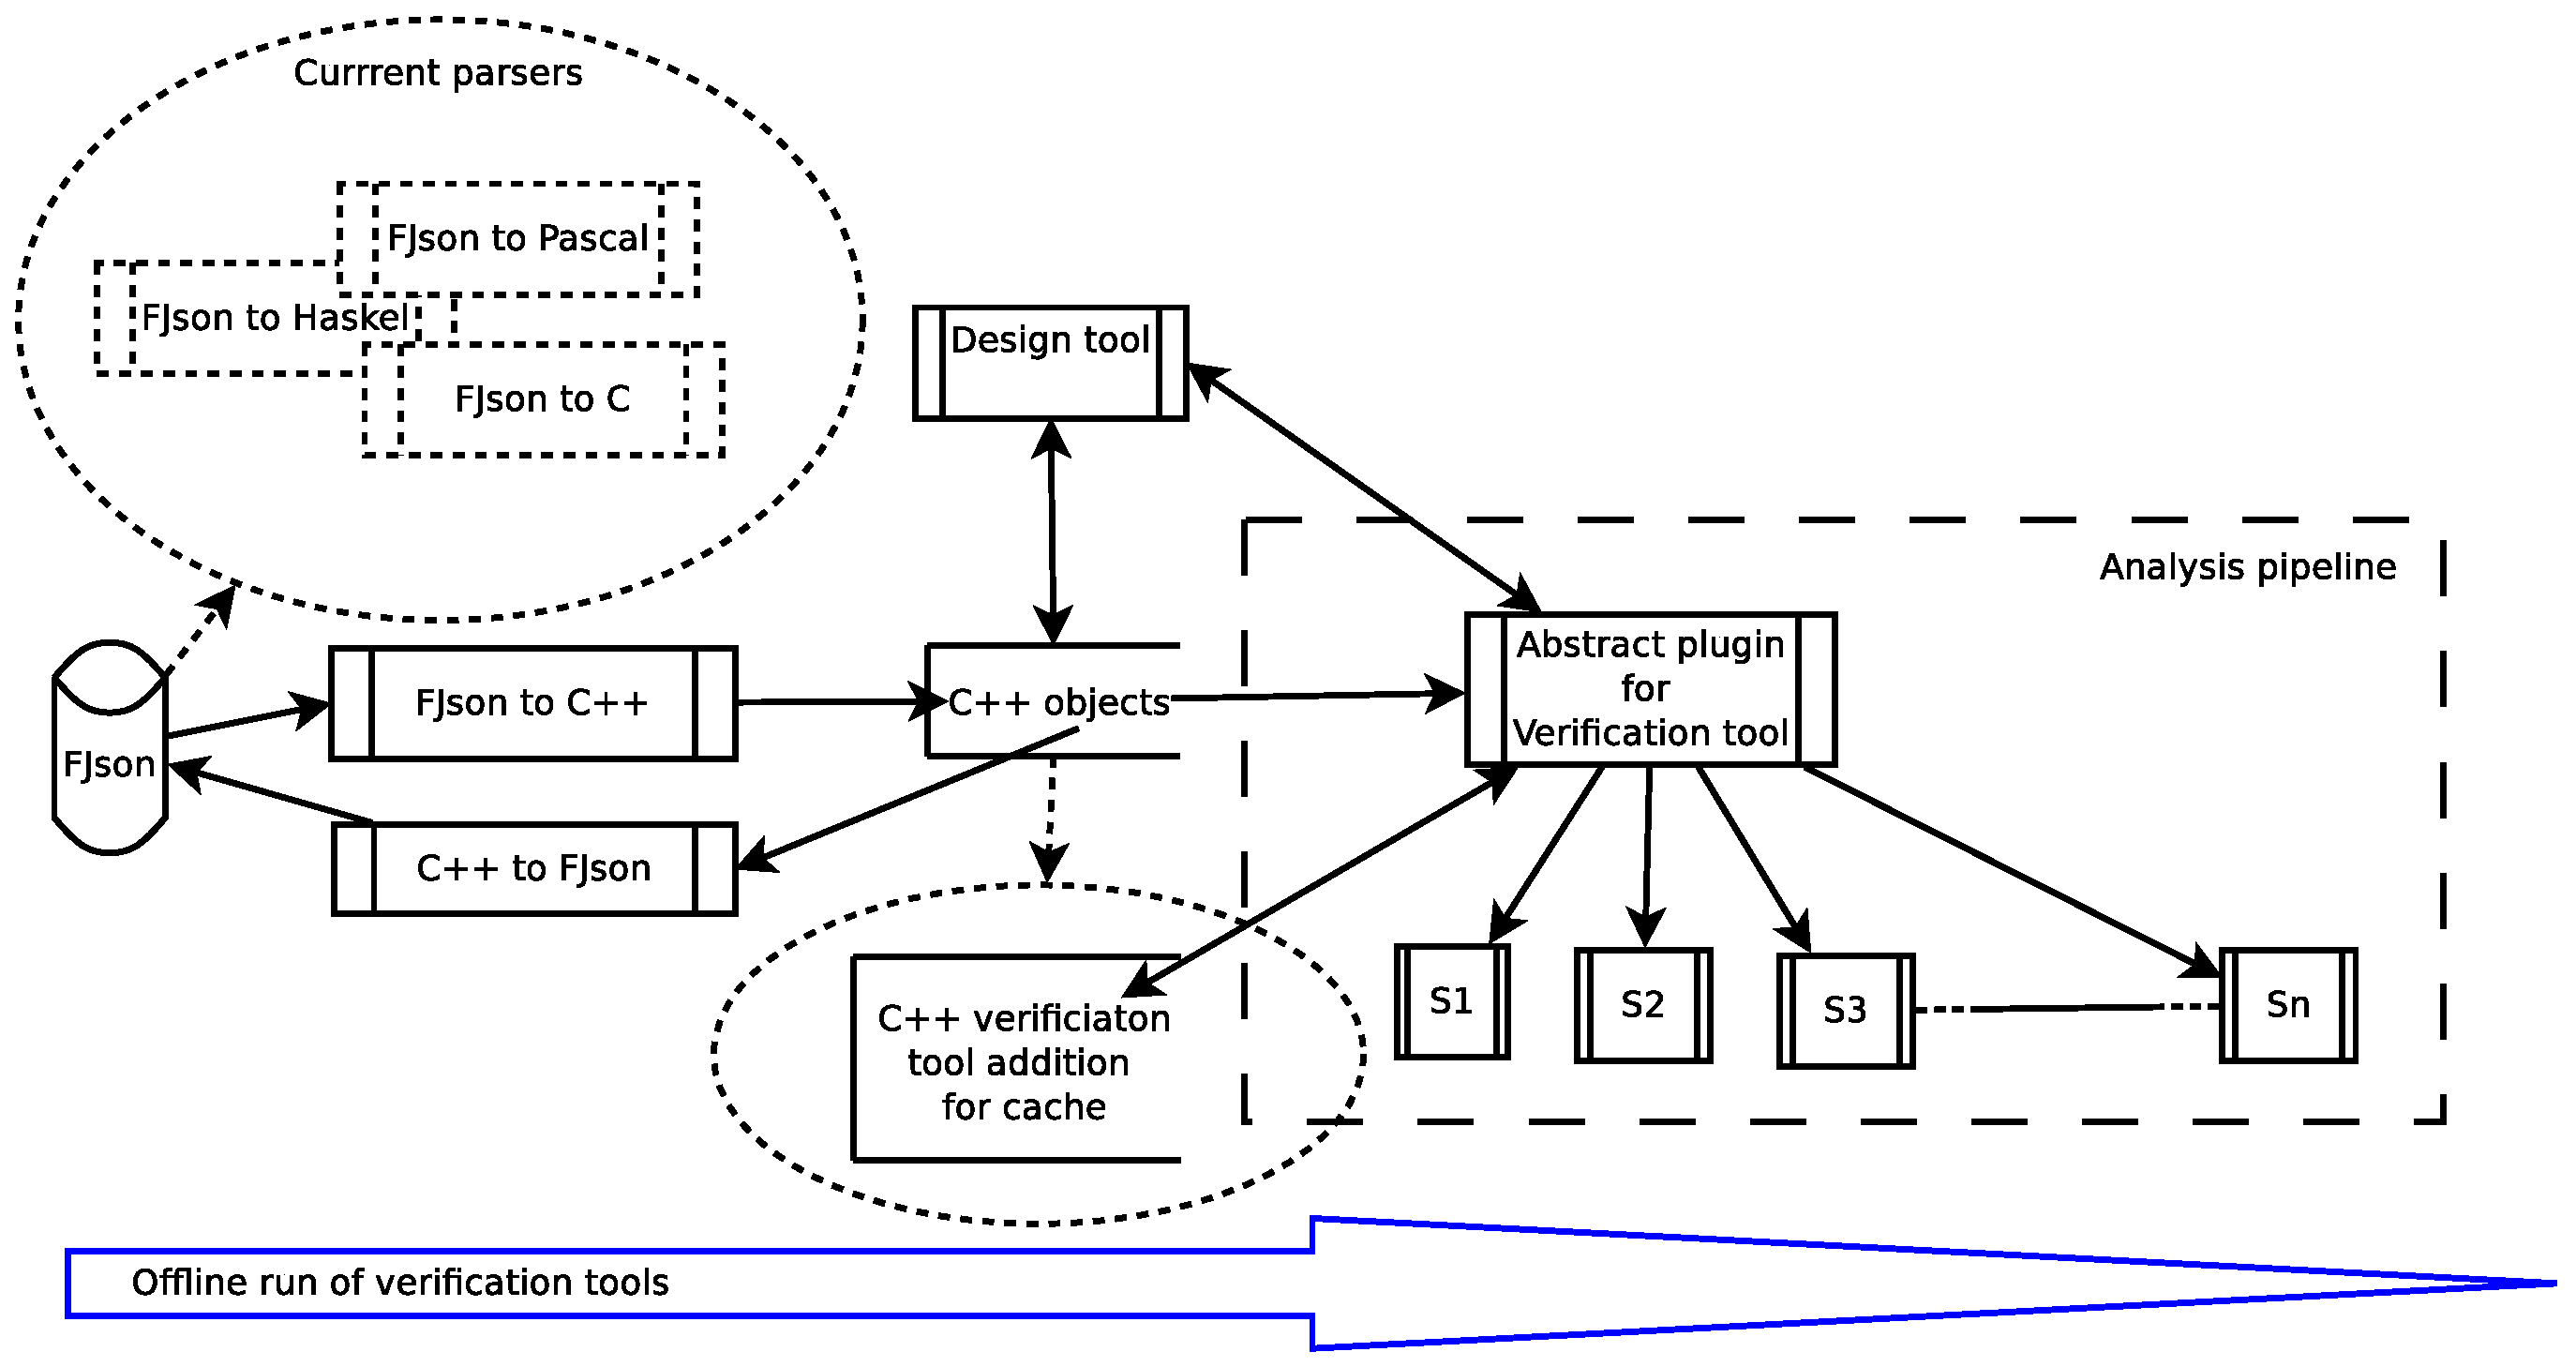
\includegraphics[width=.9\linewidth]{2014-11-27-meeting-architecture-tool}\label{}

De huidige architectuur en de gewenste architectuur van 30 km hoogte ziet er bijna identiek uit (zie 

\begin{description} 

	\item[Offline run] Een batch run van verification tools is het vanaf de
		command line draaien van de meeste of all verificatie tools op een
		model.  Bij grotere modellen duurt dit langer en wil men dit offline in
		plaats van online. Soms ook snachts.

	\item[plugin architectuur] De plugin architectuur is iets dat de verificatie
		stappen uitvoert voor 1 of meer verificatie tools. Hoe dit precies in
		elkaar zit is voor ons project buiten scope. Toch is het wel van belang, 
		omdat wij de verificatie tools moeten kunnen uitvoeren vanuit de gui.
		Binnen scope is het bouwen van een generieke plugin met zoveel mogelijk
		boilerplate code. 

	\item[Plugin communicatie] De communicatie tussen plugin en ontwerp tool
		is onderwerp van discussie. De ideeen zijn gebruik te maken van pipes 
		of van zeroMQ. Het voordeel van zeroMQ is platform onafhankelijkheid
		terwijl zeroMQ ook gebruik maakt van pipes als de processen op dezelfde
		machine draaien.
	
	\item[Current parsers] Op dit moment zijn er meerdere parsers van FJson
		naar interne structuren. Het doel van Bernard is het aantal parsers tot
		\'e\'en te beperken: die van en naar een C++ structuur. Tevens is dit
		de enige datastructuur zodat verschillen in semantiek tot het verleden
		behoren.

	\item[C++ verification tool addition] De huidige C++ datastructuur bevat
		behalve gegevens voor het model ook gegevens voor de verificatie tools.
		Het doel is voor caching zodat processing van verificatie minder lang
		duurt.  Het is ter discussie of deze gegevens in het C++ model
		thuishoren.  

\end{description}

\topic{Diverse onderwerpen}

\subtopic{Efficientere programmering}

Bernard heeft tijdens zijn promotieproject code ontwikkeld die effici\"{e}nter
omgaat met diverse C++ zaken. Dit betreft onder andere strings (een efficiente
vorm die je goedkoper kunt kopieren vergelijkbaar met bstring), en onderdelen
van de boost library. Op verzoek kan hij ons hier mee helpen.

\subtopic{}

xx


\topic{Git repository}

(open item van 15/11)
Inmiddels heeft de OU een Git server beschikbaar gemaakt. De vraag is of wij van
deze server gebruik zullen gaan maken of dat de ontwikkeling via github blijft.
Mogelijk hebben Freek en/of Bernard een voorkeur voor een private repository i.v.m.
de verspreiding van hun source code.
--> deze vraag moeten we stellen op de eerst volgende meeting met Freek en Bernard

\topic{SVN repository}
Bernard heeft ook de svn gegeven waar de C\# sources van de huidige tool te vinden
zijn. Stefan heeft deze met Vs2010 gebuild als test. 

\topic{Ontwikkelomgeving}

FLTK apps testen met VC2010 onder windows is geen probleem. 
Code Blocks daarentegen levert heel wat problemen op onder Windows XP als 8.1. 
Versie 13.12 kan niet zonder aanpassingen aan het fltk script gebruikt worden.
Bij het builden van de FLTk libraries met make van MinGW onder Code Blocks komen
er veel warnings. De documetatie README.MSWindows.txt beschrijft dat er aan
gewerkt wordt om dit op te lossen.



\topic{Repo Merging DA}
Guus heeft afgelopen week de DA branches van Stefan en zichzelf gemergt met de master.


\topic{Agile tool}
De eerder getestte agile tools werden kort overlopen en worden maandag verder besproken.  
In de loop van volgende week moeten we een keuze maken. Eens er een keuze is
maken we elk een account en gaan we experimenteren.

\topic{Demonstratie WickedXmas}

Tijdens deze demo ging het
vooral over de verificatie stappen en wat deze op de achtergrond doen.
Voor Guus kan er in de loop van volgende week een demo gegeven worden.

\topic{Vragen en afspraken}
\begin{itemize}
\item Jeroen stuurt een email naar Guus
\item maandag wordt er beslist om een afspraak te maken met Freek en Bernard i.vm.:
\begin{itemize}
\item afronden Domein analyses
\item voorstel Agile tool
\item vragen Architectuur of iteratie 0
\item ...
\end{itemize}
 \item Het volgende overleg is maandag 24 november 2014. 
\end{itemize}


\end{Minutes}
\end{document}
